\section{Experiment One: Signal Detection}
The aim of this experiment is to measure the probability of target detection for different eccentricities and surface roughness combinations. This will then give us a visibility map upon which we can base a simple model for the probability of target detection at different eccentricities and surface roughnesses.
\par
In order to carry out the 2AFC design used by \cite{najemnik-geisler2008}, the location of the target was cued for blocks of trials. This allows for (covert) attention to be deployed away from the current fixation location and to the target's location. To avoid this priming effect we will use a target/absent task where the location of the target is not known before the trial. 

\subsection{Stimuli}

A range of rough surfaces were generated by applying Lambert's cosine law to height maps generated by a $1/f^{\beta}$-noise process. For full technical details see Appendix \ref{appendix:synthesis}. The surface roughness is governed by $\beta\in\{1.60,1.65,1.70\}$ and a scaling factor, RMS roughness, which was kept constant, $\sigma_{RMS}=1.1$. For the target present trials, the target was located at one of 72 potential locations: nine different eccentricities were used $0.84^{\circ}\leq r\leq 7.5^{\circ}$, and eight evenly spaced orientations. The target was made by subtracting an ellipsoid from the three dimensional surface and subtended $0.66^{\circ}$ of visual angle. For an example, see Figure \ref{fig:smooth}.
\par
For each parameter combination, twenty different trials were created (by changing the random seed used to create the noise we can create different, yet statistically identical textured surfaces). Additionally, 160 target absent trials were included for each value of $\beta$. This gave a total of 2160 target present trials and 480 target absent. (The number of target absent trials was based on pilot results and ensured that observers made roughly equal numbers of positive and negative responses. As a large number of the target present trials were answered incorrectly we do not need so many target absent trials.)

\subsection{Method}
Two participants carried out all the trials, split into twenty subgroups, over a number of days. They were paid �50 each.  Within each subgroup of 132 trials there were 33 runs of 4 trials. During each run the participants were instructed to keep their eyes fixated on the centre of the image. Each trial consisted of a fixation cross (500ms), stimulus (200ms), white noise mask (500ms), and finally a fixation cross was displayed until a target present or absent response was given. 
\par
A Tobii x50 eyetracker was used to sample the observers' gaze every 20ms and only trials in which satisfied:
\begin{itemize}
\item the mean gaze location was within $1^{\circ}$ of the central fixation cross
\item the standard deviation of the gaze's $x$ and $y$ components was less than $2/3^{\circ}$
\end{itemize}
were included in the further analysis. 

\subsection{Results}
Trials in which fixation was not held at the centre of the image (14\%) were removed from further analysis. The results for the two individual participants are shown in Figure \ref{fig:newIndivSDRresults}. For all cases, the accuracy for the target absent trials is >90\%, and hence false positives will not be included in any further analysis. 

\begin{figure}
	\centering
		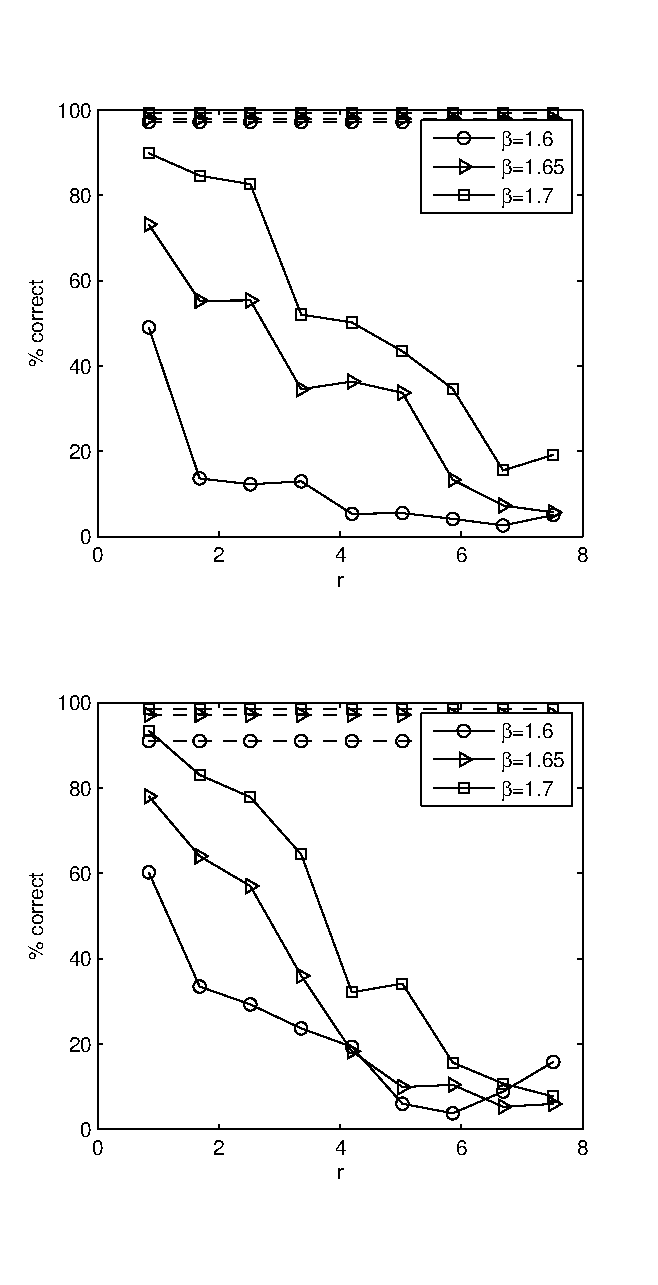
\includegraphics[width=6.5cm]{figures/newIndivSDRresults2.eps}
	\caption{Results for the two individuals from the signal detection experiment. The solid lines show the accuracy results for the target present trials, while the dashed lines shows accuracy for target absent.}
	\label{fig:newIndivSDRresults}
\end{figure}

The two subjects performed similarly and the mean target present performance is shown in Figure \ref{fig:meanRegression}. We will model this by using a simple multi-linear, with thresholding, model: 

\begin{equation}
f(\beta,r)= 4.09\beta-0.11r-5.97
$$\[ p(T|\beta,r) =  \left\{              \begin{array}{ll}                   f(\beta,r) & (f\geq0)\\                   0 & (f<0)              \end{array}       \right. \]$$
\label{linearregmodel}
\end{equation}
This regression model gives $R^2=0.934$. Note, the points $\beta=1.6,r=5.86,6.69,7.51$ were not including in the regression model. 

\begin{figure}
	\centering
		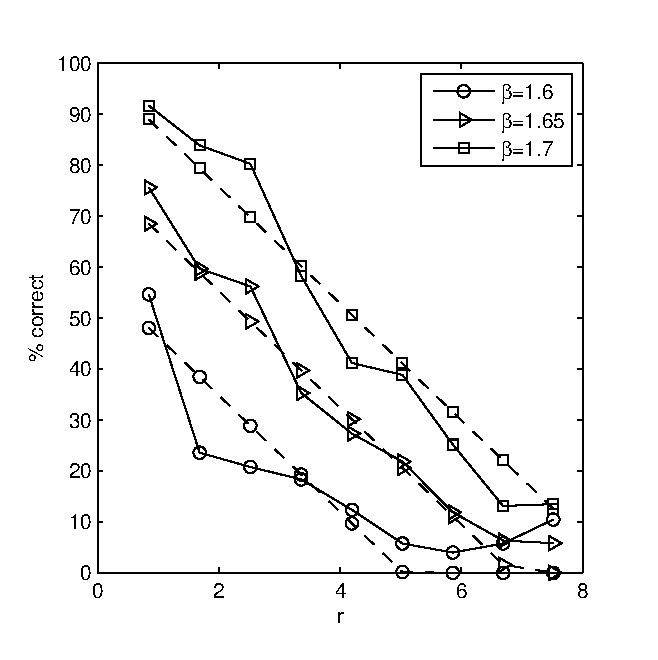
\includegraphics[width=6.5cm]{figures/meanRegression.eps}
	\caption{Solid lines show the inter-subject mean over $\beta$ and $r$ while the dashed line shows the best fit multi-linear regression.}
	\label{fig:meanRegression}
\end{figure}

